\documentclass{article}
\usepackage{graphicx}
\usepackage{float}
\graphicspath{ {./img/} }

\renewcommand{\contentsname}{Indice}
\renewcommand{\figurename}{Fig.}
\usepackage{listings}

\lstdefinestyle{mystyle}{
    basicstyle=\ttfamily\footnotesize,
    breakatwhitespace=false,         
    breaklines=true,                 
    captionpos=b,                    
    keepspaces=true,                 
    numbers=left,                    
    numbersep=5pt,                  
    showspaces=false,                
    showstringspaces=false,
    showtabs=false,                  
    tabsize=2
}

\lstset{style=mystyle}

\title{Alberi Binari di Ricerca \\
\large Confronto di diverse implementazioni
}
\author{Silviu Leonard Vatamanelu}
\date{April 2023}

\begin{document}

\maketitle
\tableofcontents
\newpage
\section{Introduzione}
Si vogliono confrontare vari modi per gestire chiavi duplicate negli Alberi Binari di Ricerca:
\begin{itemize}
    \item Implementazione senza accorgimenti particolari;
    \item Implementazione mediante flag booleano;
    \item Implementazione mediante liste.
\end{itemize}
Per raggiungere lo scopo prefissato verranno implementate le strutture dati necessarie nel linguaggio Python.

Di seguito vengono indicate come riferimento le specifiche della macchina usata per svolgere gli esperimenti:
\begin{itemize}
    \item CPU: Ryzen 5 4600U
    \item RAM: 16GB 3200MHZ
    \item OS: Windows 11 Pro 64-bit
    \item Ambiente: WSL con Ubuntu 20.04
\end{itemize}
\section{Cenni Teorici} \label{Teoria}
Un Albero binario di Ricerca è una struttura dati collegata composta da nodi. 
Ogni nodo ha 4 campi principali:
\begin{itemize}
    \item Key: il valore rispetto al quale viene deciso il posizionamento di un nodo;
    \item Left: un puntatore al figlio sinistro;
    \item Right: un puntatore al figlio destro;
    \item Parent: un puntatore al padre.
\end{itemize}
Per memorizzare un Albero binario di Ricerca è quindi necessario mantenere il del nodo radice (Root) il quale avrà il campo Parent impostato a NIL.
La proprietà principale dell'Albero binario di Ricerca è l'ordinamento: all'interno del sottoalbero sinistro di un qualsiasi nodo si hanno Key con valore inferiore o uguale a quello del nodo, mentre all'interno del sottoalbero destro si trovano solo Key con valore superiore o uguale a quello del nodo.
L'inserimento all'interno di un Albero binario di Ricerca avviene quindi confrontando la propria Key con quella della Root, se il valore è minore o uguale si ripete la procedura nel sottoalbero sinistro altrimenti in quello destro, fino a che non si trova un NIL.
Il punto di critico di questa procedura è l'inserimento delle chiavi duplicate.
Esistono varie strategie per la loro gestione, vengono riportate solo quelle di interesse:
\begin{itemize}
    \item Normale: si sceglie arbitrariamente un sottoalbero;
    \item Flag booleano: ogni nodo ha un campo aggiuntivo Flag che tiene traccia dell'ultimo sottoalbero visitato per l'inserimento;
    \item Liste: ogni nodo contiene una lista dove verrano inseriti tutti gli elementi con chiave uguale.
\end{itemize}
Ognuna delle implementazioni presenta vabtaggi e criticità: 
l'implementazione normale rende l'albero sbilanciato perché tutti i nodi uguali finiscono nello stesso sottoalbero, e nel caso in cui tutte le chiavi siano uguali si ha una lunga catena, in compenso è di semplice implementazione;
l'implementazione mediante liste asintoticamente perde i vantaggi dell'Albero binario di Ricerca e somiglia più a una lista concatenata, in compenso le operazioni di cancellazione e inserimento sono estremamente semplici; mentre l'implementazione con flag garantisce un migliore bilanciamento dell'albero al costo di complicare l'operazione di rimozione di un nodo.
Per apprezzare quindi le differenze tra le possibili implementazioni degli Alberi Binari di Ricerca bisogna concentrarsi su 3 aspetti fondamentali: Inserimento, Cancellazione e Bilanciamento dell'Albero.
\section{Descrizione degli esperimenti} \label{esperimenti}
In seguito alle considerazioni svolte nella sezione \ref{Teoria} si ritiene necessario eseguire degli esperimenti sui seguenti metodi e sulle seguenti proprietà per confrontare le prestazioni delle 3 implementazioni:
\begin{enumerate}
    \item Inserimento di nodi
    \item Rimozione di nodi
    \item Ricerca di un nodo
    \item Profondità dell'albero
\end{enumerate}
Gli esperimenti saranno quindi strutturati come segue:
Per ogni implementazione di Albero binario di ricerca viene effettuato l'inserimento di un numero compreso tra \( [10, 10000] \) nodi con passo 50 e con chiavi estratte casualmente all'interno degli intervalli \( [0, 100]\) e \( [0, 500]\). Tali intervalli vengono scelti in modo da avere sempre una buona probabilità di ottenere chiavi duplicate. Viene calcolata la profondità dell'albero, e successivamente si effettua la ricerca di un numero di chiavi pari a \( \lfloor len(ABR.length) / 4 \rfloor \) scelte casualmente dai valori inseriti nell'albero e la rimozione di tali elementi. Al termine viene calcolata nuovamente la profondità dell'albero. 

Gli esperimenti vengono ripetuti 100 volte per ogni intervallo e lunghezza dell'albero; dei dati con stesso tipo di implementazione e lunghezza dell'albero viene fatta la media e poi i dati risultanti vengono mostrati sotto forma di grafico. 
\section{Documentazione del codice}

\begin{figure}[h!] \label{uml}
\centering
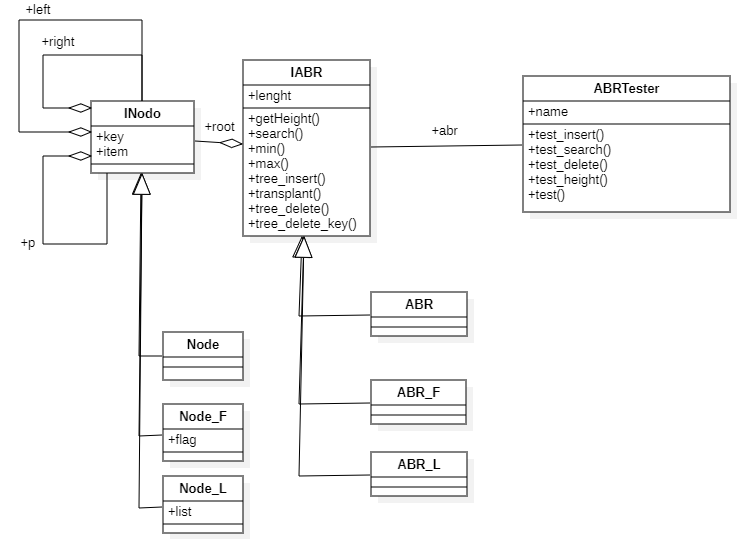
\includegraphics[width=\textwidth]{uml}
\caption{Diagramma UML}
\end{figure}

La figura \ref{uml} rappresenta il diagramma delle classi utilizzato per la soluzione. È importante notare che nell'implementazione del codice, ogni derivazione di IABR implementa la relativa derivazione di INode a lui compatibile, quindi ABR utilizzerà la classe Node, ABR\_F utilizzerà Node\_F e ABR\_L utilizzerà Node\_L. Nelle varie implementazioni cambiano soltanto le operazioni effettuate dai metodi \verb| tree_insert(), tree_search(), tree_delete_key() | nei quali cambia la gestione del nodo di riferimento.
\subsection{Inserimento}
Ogni implementazione comprende i metodi \verb|tree_insert() e __tree_insert()|.
Il primo si ocupa di creare un nuovo nodo a partire dai dati in input e richiamare il secondo.
L'algoritmo di inserimento, infatti, è interamente contenuto in \verb|__tree_insert()| di cui si riporta l'implementazione nel frammento \ref{inserimentobase}. \newpage

\begin{lstlisting}[language=Python, caption={Algoritmo di inserimento base}, label=inserimentobase]
    def __tree_insert(self, z: Node):
        # Inserisce un nodo z all'interno dell'albero
        y = None
        x = self.root
        while x is not None:
            y = x
            if z.key < x.key:
                x = x.left
            else:
                x = x.right
        z.p = y
        if y is None:
            self.root = z
        elif z.key < y.key:
            y.left = z
        else:
            y.right = z
        self.length += 1
\end{lstlisting}

Tale algoritmo è implementato all'interno della classe ABR.
ABR\_F e ABR\_L, rispetto alla variante base presentano delle variazioni alla prima della riga 7 e della riga 14 , indicate nei frammenti seguenti con dei commenti.

\begin{lstlisting}[language=Python, caption={Algoritmo di inserimento nell'implementazione con Lista}, label=inserimentolista]
    ## riga 7
    if z.key == x.key:
        break
    ##riga 14
    elif z.key == y.key:
        y.list.append(z)
\end{lstlisting}

Nel frammento \ref{inserimentolista}, prima della riga 7 del frammento \ref{1} viene inserito un controllo di uguaglianza per fermare la discesa all'interno dell'albero per la ricerca  di un figlio vuoto per l'inserimento, in quanto ogni nodo mantiene una lista di tutti i nodi con chiave uguale. Ciò significa che dobbiamo inserire all'interno della lista del nodo y l'elemento z appena creato, come mostrato dal codice da inserire prima della riga 14.

\begin{lstlisting}[language=Python, caption={Algoritmo di inserimento nell'implementazione con flag}, label=inserimentoflag]
    ##riga 7
    if z.key == x.key:
        # Controllo il flag con logica inversa per decidere se inserire il nodo nel sottoalbero sinistro o destro
        if x.flag:
            x = x.right
        else:
            x = x.left
        # se l'inserimento non avviene al prossimo livello, cambio il flag in modo da bilanciare i molti valori ripetuti
        if x is not None:
            y.flag = not y.flag
    ##riga 14
    elif z.key == y.key:
        # Controllo il flag per decidere se inserire il nodo nel sottoalbero sinistro o destro del padre
        if y.flag:
            y.right = z
        else:
            y.left = z
        # Cambio il flag
        y.flag = not y.flag
\end{lstlisting}
Nel frammento \ref{inserimentoflag}, prima della riga 7 del frammento \ref{1} viene inserito un controllo di uguaglianza perdecidere in quale sottoalbero proseguire la ricerca, in quanto ogni nodo mantiene un flag che indica la direzione. Viene poi inserito un controllo per evitare di scendere nell'albero e trovare all'altezza successiva un 'posto' per l'inserimento in modo da non cambiare 2 volte il flag del padre. Nel codice da inserire prima della riga 14 viene controllato il flag del padre e viene deciso il figlio in cui eseguire l'inserimento.

\subsection{Ricerca}
Ogni implementazione della ricerca comprende i metodi \verb|search() e __search()|.
Il primo si occupa chiamare il secondo a partire dalla radice dell'albero con la chiave da cercare.
L'algoritmo di ricerca, infatti, è interamente contenuto in \verb|__search()| di cui si riporta l'implementazione nel frammento \ref{inserimentobase}.

\begin{lstlisting}[language=Python, caption={Algoritmo di ricerca base}, label=ricercabase]
    def __search(self, x: Node, k: int) -> Node:
        # Metodo ricorsivo che cerca un nodo con chiave k nell'albero
        if x is None or x.key == k:
            return x
        if k < x.key:
            return self.__search(x.left, k)
        else:
            return self.__search(x.right, k)
\end{lstlisting}

Tale algoritmo è implementato all'interno della classe ABR e ritorna il primo nodo con chiave k.
ABR\_F e ABR\_L, rispetto alla variante base non presentano variazioni in quanto la ricerca si ferma alla prima occorrenza quindi non è necessario prevedere accorgimenti particolari. Diverso sarebbe per una ricerca completa di tutte le chiave, in quanto l'algoritmo base dovrebbe tenere traccia dei nodi incontrati e continuare la ricerca in un singolo sottoalbero dato che l'inserimento avviene sempre nel sottoalbero destro. Per quanto riguarda l'implementazione con flag la ricerca deve avvenire in entrambi i sottoalberi in quanto non siamo a conoscenza del numero di occorrenze della chiave duplicata, mentre la variante con lista non richiede accorgimenti aggiuntivi per laricerca del nodo, ma la ricerca di un elemento specifico deve poi avvenire nella lista.

\subsection{Cancellazione}
Ogni implementazione comprende i metodi \verb|tree_delete(), transplant()| e \verb|tree_delete_key()|.
I primi due cancellano un nodo ed evitano l'inconsistenza dell'albero, mentre l'ultimo effettua l'eliminazione di tutti i nodi con chiave uguale. Di seguito l'implementazione per l'albero normale.

\begin{lstlisting}[language=Python, caption={Algoritmo di eliminazione base}, label=inserimentobase]
       def transplant(self, u: Node, v: Node):
        # Sostituisce il nodo u con il nodo v
        if u.p is None:
            self.root = v
        elif u == u.p.left:
            u.p.left = v
        else:
            u.p.right = v
        if v is not None:
            v.p = u.p

    def tree_delete(self, z: Node):
        # Elimina il nodo z dall'albero
        if z.left is None:
            self.transplant(z, z.right)
        elif z.right is None:
            self.transplant(z, z.left)
        else:
            y = self.min(z.right)
            if y.p != z:
                self.transplant(y, y.right)
                y.right = z.right
                y.right.p = y
            self.transplant(z, y)
            y.left = z.left
            y.left.p = y

        self.length -= 1
        
    def tree_delete_key(self, key: int):
        z = self.search(key)
        self.__tree_delete_key(key, z)

    def __tree_delete_key(self, key: int):
        v = node.right
        if v is not None and v.key == key:
            self.__tree_delete_key(key, v)
        self.tree_delete(node)   
\end{lstlisting}

In \verb|__tree_delete_key()| per eliminare tutte le occorrenze di una chiave è sufficiente controllare il sottoalbero destro.
ABR\_F e ABR\_L, rispetto alla variante base presentano delle variazioni soltanto nel metodo \verb
tree_delete_key() di cui vengono riportate le mdifiche.

\begin{lstlisting}[language=Python, caption={Algoritmo di eliminazione nell'implementazione con Lista}, label=cancellazionelista]
    def tree_delete_key(self, key: int):
        z = self.search(key)
        if z is not None:
            self.tree_delete(z)
\end{lstlisting}

Nel frammento \ref{cancellazionelista}, non è necessario il metodo ausiliario ricorsivo per cercare tutte le occorrenze dato che si trovano tutte all'interno dello stesso nodo. È sufficiente quindi cancellare solo il nodo z.

\begin{lstlisting}[language=Python, caption={Algoritmo di eliminazione nell'implementazione con flag}, label=eliminazioneflag]
    def __tree_delete_key(self, key: int, node: None) -> bool:
        # Elimina i nodo con chiave k dall'albero, per ini
        if node is None:
            return
        else:
            if node.flag:
                u = node.left
                v = node.right
            else:
                u = node.left
                v = node.right

            if u is not None and u.key == key:
                self.__tree_delete_key(key, u)
            if v is not None and v.key == key:
                self.__tree_delete_key(key, v)
            self.tree_delete(node)              
\end{lstlisting}
Nel frammento \ref{eliminazioneflag}, come nel caso della ricerca devono essere controllati entrambi i sottoalberi in quanto non abbiamo informazioni riguardo all'occorrenza dei duplicati.
Possiamo velocizzare l'algoritmo iniziando l'eliminazione dal sottoalbero in cui è stato effettuato l'ultimo inserimento.

Per brevità non si riportano le implementazioni di \verb|max(), min()| e \verb|getHeight()|.
\subsection{Test} \label{test}
La classe ABRTester implementa le procedure per registrare i tempi e l'altezza dell'albero in seguito alle varie operazioni.
Si riporta il codice usato nel metodo test: 
\begin{lstlisting}[language=Python, caption={Algoritmo di test}, label=eliminazioneflag]
    def test(self, values: list) -> pd.DataFrame:
        # colonne: n, abr_type, height_before, height_after, insert_time, search_time, delete_time
        # righe: 1 riga per ogni test
        n = len(values)
        # inserimento dei valori nell'albero
        insert_times = []
        for v in values:
            insert_times.append(self.test_insert(v, chr(v)))
        insert_df = pd.DataFrame(insert_times)
        height_before = self.test_height()
        # ricerca dei valori nell'albero
        search_times = []
        values2 = np.random.choice(values, int(np.floor(n / 4)))
        for v in values2:
            search_times.append(self.test_search(v))
        search_df = pd.DataFrame(search_times)
        # eliminazione dei valori dall'albero
        delete_times = []
        for v in values2:
            delete_times.append(self.test_delete(v))
        delete_df = pd.DataFrame(delete_times)
        height_after = self.test_height()
        # creazione del dataframe
        return pd.DataFrame({
            'n': n,
            'abr_type': self.type,
            'height_before': height_before,
            'height_after': height_after,
            'insert_time': insert_df.mean(),
            'search_time': search_df.mean(),
            'delete_time': delete_df.mean()
        })     

    def test_delete(self, key: int) -> float:
        start = perf_counter()
        self.ABR.tree_delete_key(key)
        end = perf_counter()
        return end - start
    
    def test_height(self) -> int:
        return self.ABR.getHeight(self.ABR.root)
\end{lstlisting}
I metodi \verb|test_insert()| e \verb|test_search()| non vengono riportati in quanto del tutto simili a \verb|test_delete()|.
Il codice fa quanto descritto nella sezione \ref{esperimenti}: inserisce n valori e registra il tempo di ognuno attraverso dei \verb|perf_counter()|, viene poi calcolata l'altezza dell'albero. Vengono scelti dei valori casuali tra quelli inseriti per effettuare la ricerca e poi la cancellazione, e viene registrata l'altezza dell'albero in seguito alla cancellazione.
I dati vengono restituiti sotto forma di DataFrame contente la media dei tempi. Viene scelta la media in modo da poter analizzare gli algoritmi nel loro complesso in quanto la scelta dei massimi avrebbe portato a tempi influenzati dalle ultime operazioni eseguite in inserimento e dalla posizione nell'albero per l'eliminazione e la ricerca. Viceversa per il minimo: Il primo inserimento è quello con tempo minimo mentre la ricerca e l'eliminazione hanno il tempo minimo se il valore si trova "in alto" nell'albero e non ci sono altri valori.

L'operazione di test viene ripetuta dal main del programma che viene riportato nel frammento numero \ref{listtest}.

\begin{lstlisting}[language=Python, caption={Algoritmo di test}, label=listtest]
RANDOM_RANGES = [(0, 100), (0, 500)]
DATA_MEAN = 100
ITERATIONS = (10, 10000)
STEP = 50
for random_range in RANDOM_RANGES:
    df_list: list = []
    for d in range(DATA_MEAN):
        df_app: list = []
        value_list: list = []
        for i in range(ITERATIONS[0], ITERATIONS[1], STEP):
            value_list.append(np.random.randint(random_range[0], random_range[1], i))
        for i in range(ITERATIONS[0], ITERATIONS[1], STEP):
            df_app.append(ABRTester(lista.ABR(), 'lista').test(value_list[(i - ITERATIONS[0]) // STEP]))
        for i in range(ITERATIONS[0], ITERATIONS[1], STEP):
            df_app.append(ABRTester(flag.ABR(), 'flag').test(value_list[(i - ITERATIONS[0]) // STEP]))
        for i in range(ITERATIONS[0], ITERATIONS[1], STEP):
            df_app.append(ABRTester(abr.ABR(), 'abr').test(value_list[(i - ITERATIONS[0]) // STEP]))

        print(f'{d} - {random_range[1]}')
        df_list.append(pd.concat(df_app, ignore_index=True))

    df_concat = pd.concat(df_list)
    by_row_index = df_concat.groupby([df_concat.index, 'n', 'abr_type'])
    df = by_row_index.mean(numeric_only=True).reset_index()
    # salvataggio dei grafici omesso
\end{lstlisting}
Viene riportato il codice per puntualizzare l'otternimento dei dati:
Il ciclo esterno viene eseguito su ogni intervallo da cui vengono scelti i numeri casuali;
il ciclo interno esegue \verb|DATA-MEAN| volte la generazione dei dati, e il test di ogni implementazione su quei dati. I cicli più interni sono separati per una più semplice lettura del DataFrame risultante, ogni test però lavora sugli stessi dati in ingresso generati prima dei test.
I dati risultanti vengono concatenati e raggruppati per dimensione e tipo di albero e viene effettuata una media dei valori così ottenuti. Il DataFrame finale viene poi rappresentato sottoforma di grafico in tutte le sue parti con l'asse y in scala logaritmica.
\section{Risultati degli esperimenti}
In questa sezione verranno riportati i grafici per tutte le informazioni ottenute dall'esecuzione degli algoritmi secondo le modalità descritte nelle sezioni \ref{esperimenti} e \ref{test}.
\subsection{Inserimento}
Da questo esperimento ci aspettiamo un comportamento simile per le implementazione normale e con flag, proporzianale all'altezza dell'albero i.e. \( O(h) \). Mentre un comportamento inizialmente simile per la rimanente implementazione ma poi peggiore dovuto ai tanti duplicati e all'inseriemento sequenziale nella lista. Ci aspettiamo dall'intervallo più ampio un minore calo di prestazioni per la lista.
\begin{figure}[H]
\centering
  \centering
  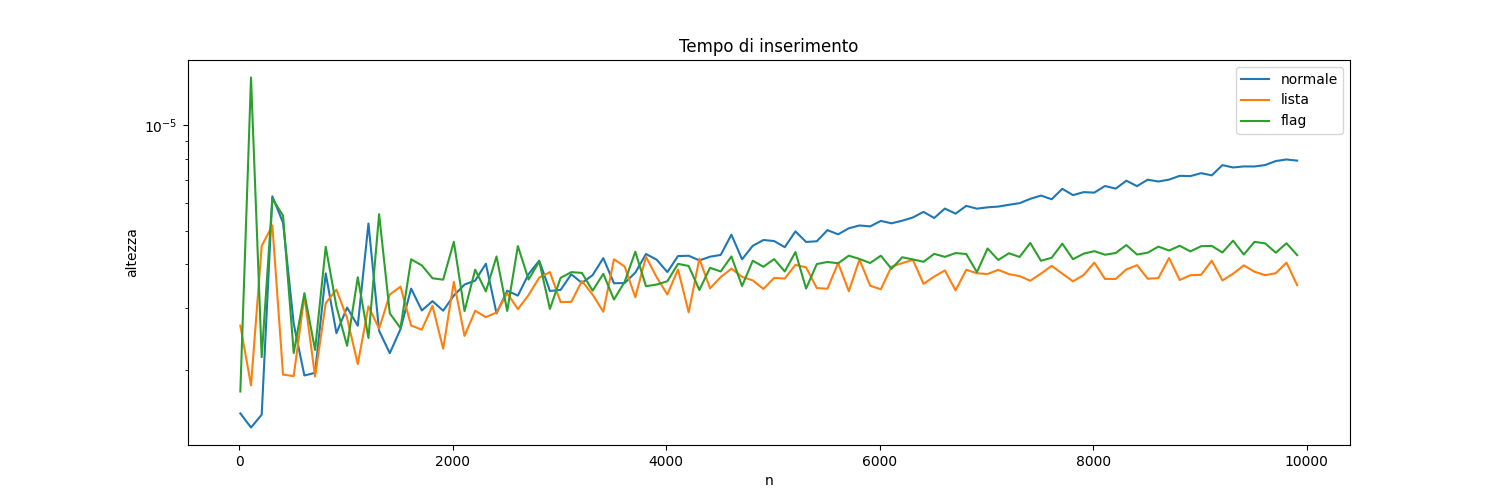
\includegraphics[width=\linewidth]{img/insert_graph_100_log.png}
  \caption{Tempo di inserimento con intervallo  \( [0, 100] \) }
  \label{insert100}
\end{figure}
\begin{figure}[H]
\centering
  \centering
  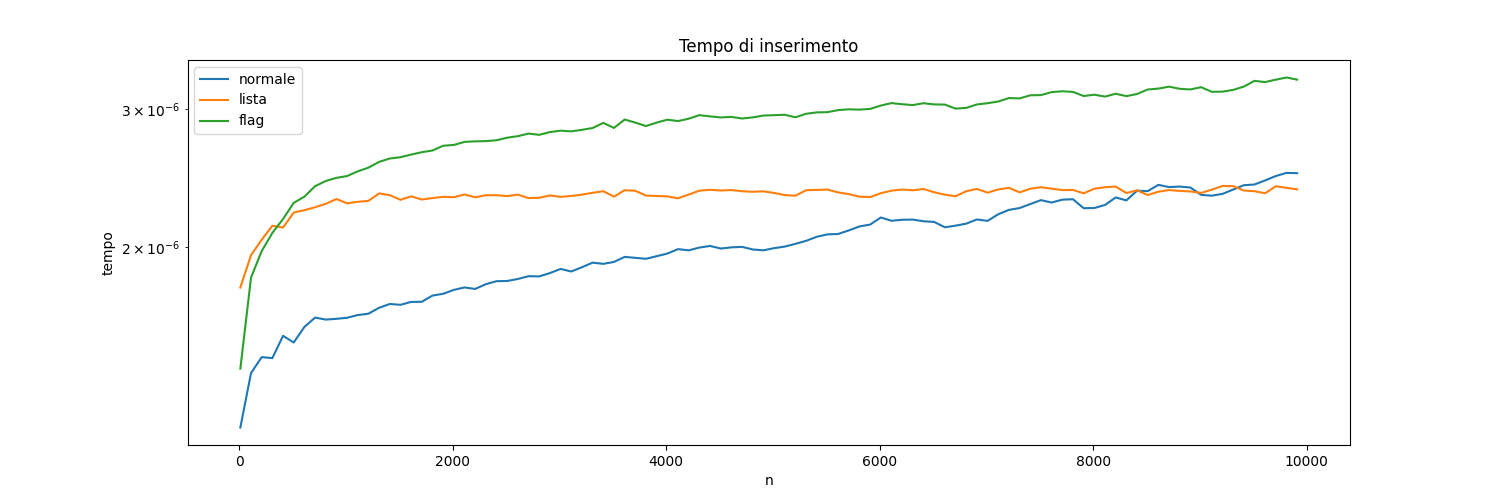
\includegraphics[width=\linewidth]{img/insert_graph_500_log.png}
  \caption{Tempo di inserimento con intervallo \( [0, 500] \) }
  \label{insert500}
\end{figure}
I risultati rappresentati nelle figure \ref{insert100} e \ref{insert500} confermano parzialmente quanto intuito: l'implemezione mediante liste non peggiora all'aumentare della dimensione dell'albero; ciò e probabilmente dovuto all'implementazione del metodo \verb|append()| in Python. 
Le tempistiche per le implementazioni con flag e normale, invece, seguono un andamento molto simile.
\subsection{Altezza prima dell'eliminazione}
Da questo esperimento ci aspettiamo di vedere i risultati peggiori per l'implementazione normale, mentre i migliori per l'implementazione con le liste. Questo perchè l'altezza dell'albero, per inserimenti casuali, va come \( O(\log n) \) dove n è il numero di chiavi uniche, quindi l'implementazione a liste è avvantaggiata in quanto tratta le chiavi come univoche e le duplicate risiedono nello stesso nodo. Tra l'implementazione normale e quella con i flag, possiamo aspettarci risultati migliori dalla seconda in quanto cerca di bilanciare i valori duplicati.
\begin{figure}[H]
\centering
  \centering
  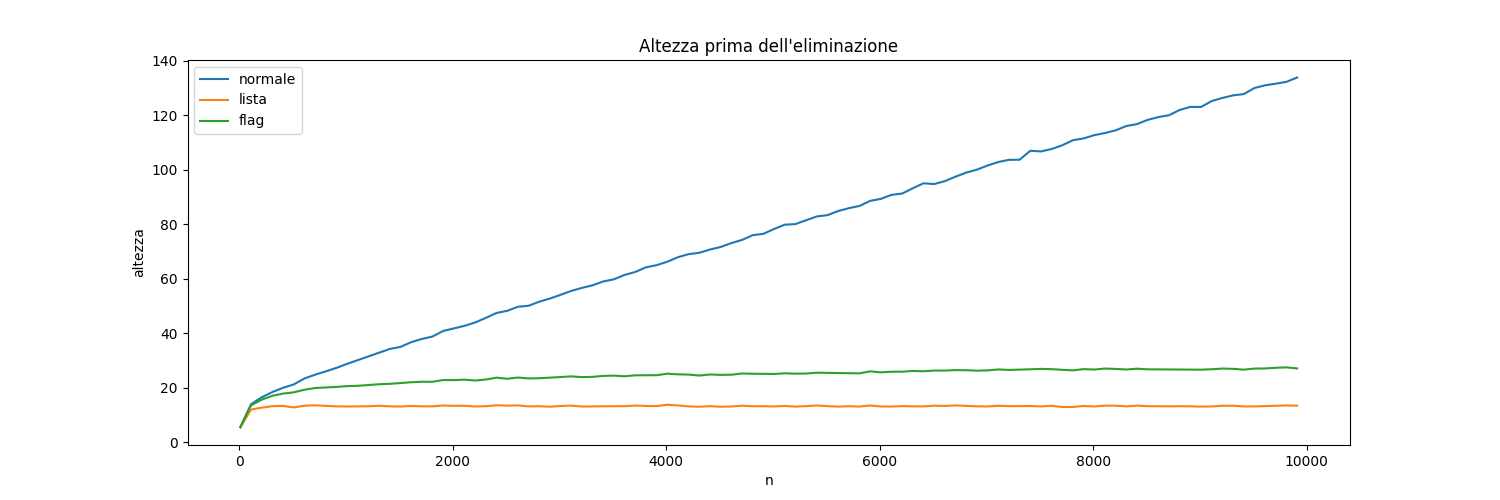
\includegraphics[width=\linewidth]{img/height_before_graph_100_linear.png}
  \caption{Altezza con intervallo \( [0, 100] \) }
  \label{before100}
\end{figure}
\begin{figure}[H]
\centering
  \centering
  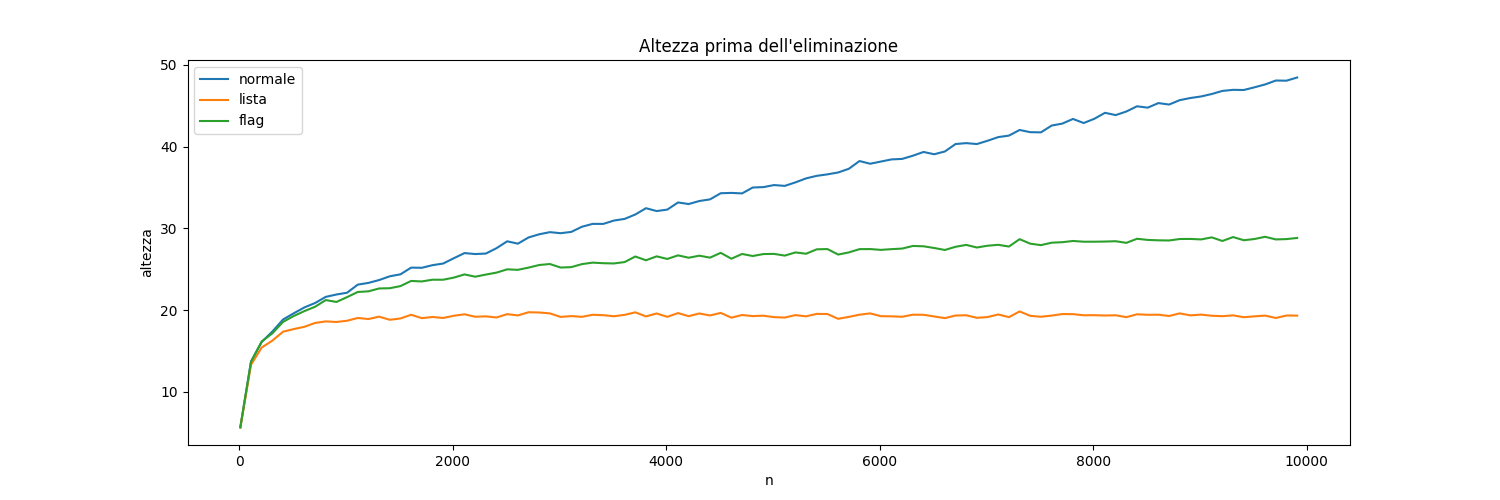
\includegraphics[width=\linewidth]{img/height_before_graph_500_linear.png}
  \caption{Altezza con intervallo \( [0, 500] \) }
  \label{before500}
\end{figure}
I risultati rappresentati nelle figure \ref{before100} e \ref{before500} confermano quanto intuito: l'implemezione mediante liste risulta piu efficace in quanto ha un altezza al piu pari al logaritmo dell'estremo superiore dell'intervallo utilizzato. Invece, le altre due implementazioni vengono influenzate dalle numerose chiavi duplicate presenti.
\subsection{Ricerca}
Dato che la ricerca viene effettuata sul primo elemento con chiave uguale, ci aspettiamo un andamneto molto simile per tutte le implementazioni, diverso caso per la ricerca di tutti gli elementi. Dato che la ricerca viene effettuata per chiave e non per valore, non si riescono a riscontrare gli svantaggi dell'implementazione con liste. 
\begin{figure}[H]
\centering
  \centering
  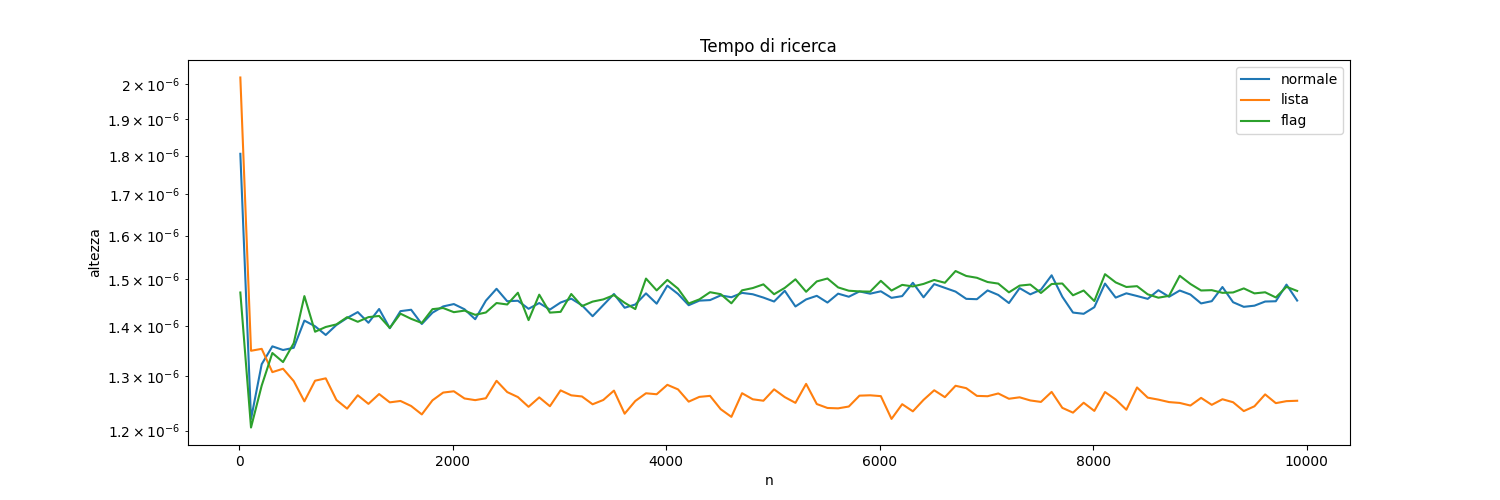
\includegraphics[width=\linewidth]{img/search_graph_100_log.png}
  \caption{Tempo di ricerca con intervallo  \( [0, 100] \) }
  \label{search100}
\end{figure}
\begin{figure}[H]
\centering
  \centering
  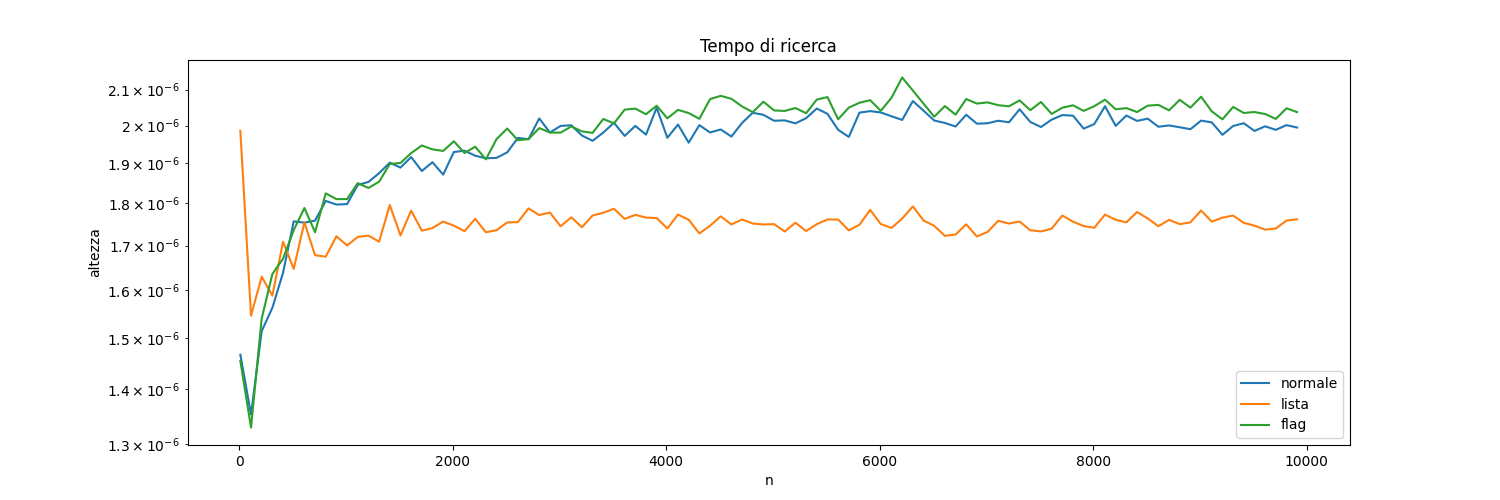
\includegraphics[width=\linewidth]{img/search_graph_500_log.png}
  \caption{Tempo di ricerca con intervallo \( [0, 500] \) }
  \label{search500}
\end{figure}
I risultati rappresentati nelle figure \ref{search100} e \ref{search500} confermano quanto intuito: le implementazioni condividono tempistiche molto simili. 
L'implementazione mediante liste risulta però leggermente migliore in quanto l'albero che ne risulta è piu basso.
\subsection{Eliminazione}
Da questo esperimento ci aspettiamo un comportamento simile per le implementazione normale e con flag, proporzianale all'altezza dell'albero i.e. \( O(h) \). Mentre risultati simili alla ricerca per l'implemetazione con liste. Anche in questo caso è da notare che l'eliminazione è per chiave e non per valore quindi viene eliminato il costo della ricerca del valore corretto nella lista dei nodi duplicati.
\begin{figure}[H]
\centering
  \centering
  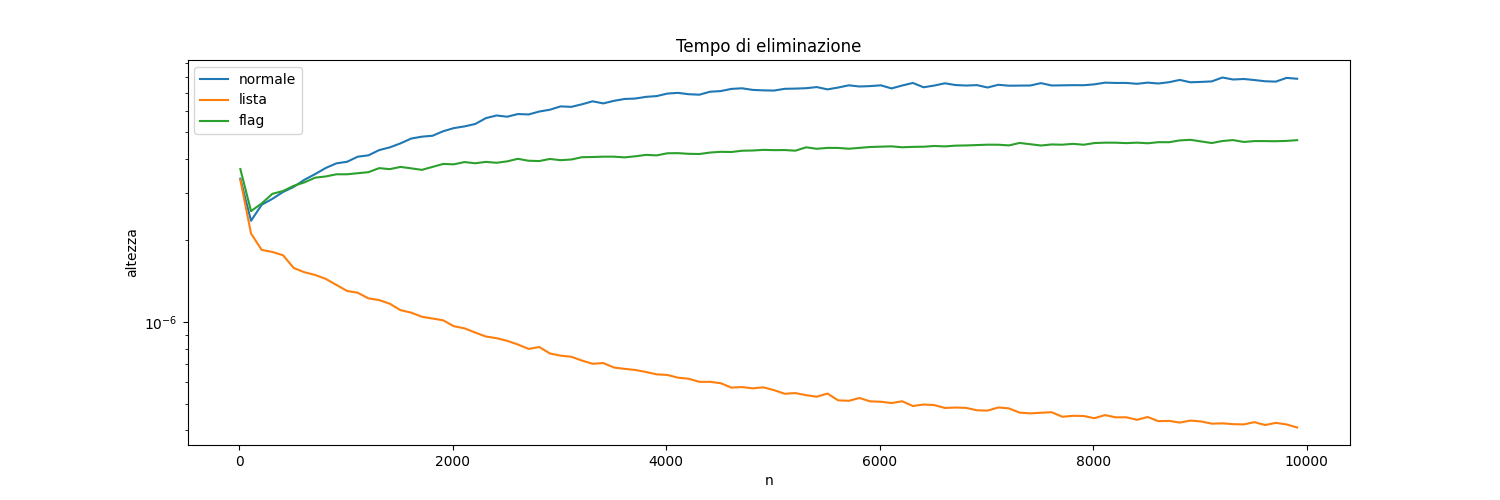
\includegraphics[width=\linewidth]{img/delete_graph_100_log.png}
  \caption{Tempo di eliminazione con intervallo \( [0, 100] \) }
  \label{delete100}
\end{figure}
\begin{figure}[H]
\centering
  \centering
  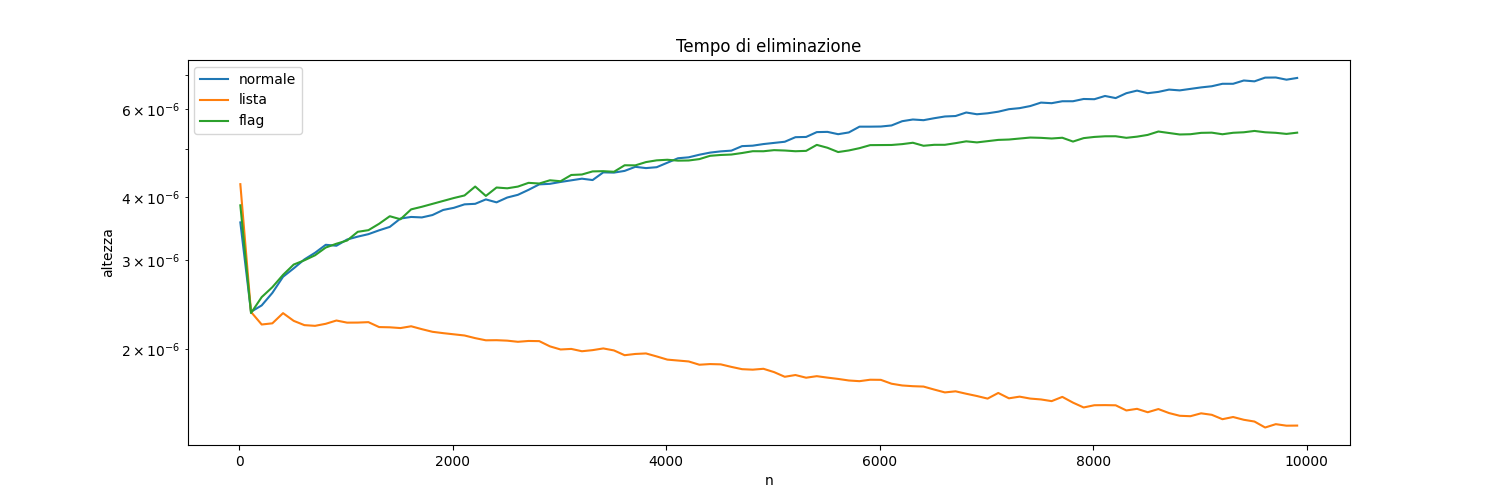
\includegraphics[width=\linewidth]{img/delete_graph_500_log.png}
  \caption{Tempo di eliminazione con intervallo \( [0, 500] \) }
  \label{delete500}
\end{figure}
I risultati rappresentati nelle figure \ref{delete100} e \ref{delete500} confermano quanto intuito: l'implemezione risulta migliore delle altre due per la minore altezza dell'albero risultante. La componente costante verso la coda di tutte e tre le curve è dovuta allo svuotamento dell'albero e al conseguente tempo costante per la ricerca della chiave da eliminare.
\subsection{Altezza dopo l'eliminazione}
Questo esperimento viene eseguito per ottenere delle informazioni riguardo uno scenario tipico di utilizzo della struttura dati in cui un utente effettua degli inserimenti e poi delle cancellazioni. L'altezza in seguito a questo scenario è rilevante perchè influenza le operazioni successive.
Da questo esperimento ci aspettiamo di vedere una decrescita lineare per l'implementazione a liste, mentre un andamento più irregolare per le altre due implementazioni.
\begin{figure}[H]
\centering
  \centering
  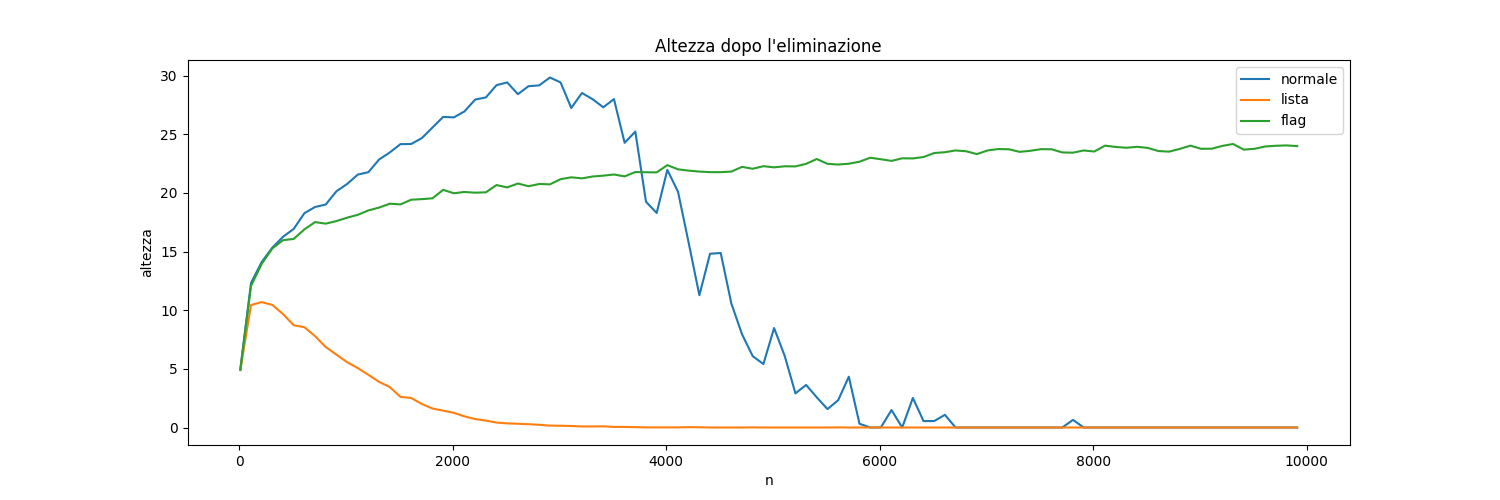
\includegraphics[width=\linewidth]{img/height_after_graph_100_linear.png}
  \caption{Altezza con intervallo \( [0, 100] \) }
  \label{after100}
\end{figure}
\begin{figure}[H]
\centering
  \centering
  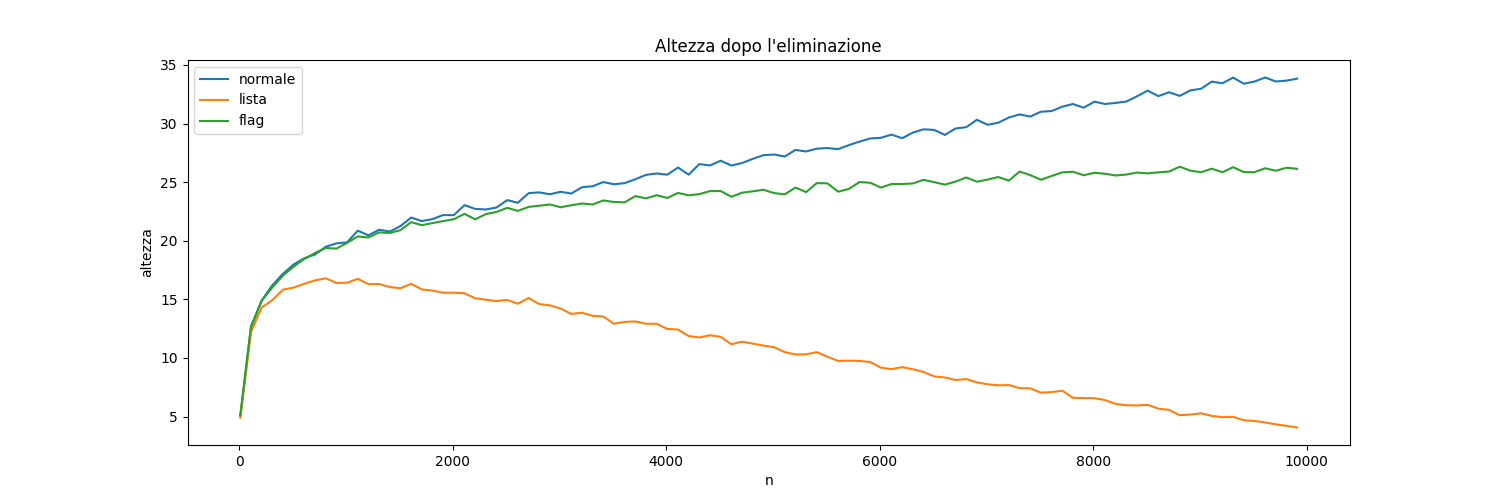
\includegraphics[width=\linewidth]{img/height_after_graph_500_linear.png}
  \caption{Altezza con intervallo \( [0, 500] \) }
  \label{after500}
\end{figure}
I risultati rappresentati nelle figure \ref{after100} e \ref{after500} confermano parzialmente quanto intuito: l'implemezione mediante liste decresce velocemente. I valori tra 0 e 1 sono dovuti alla casualità dei numeri generati e sono chiaramente dovuti all'intervallo usato e al metodo di scelta dei valori da cancellare.
Risulta poco comprensibile l'andamento i figura \ref{after100} della variante con flag il quale sembra non effettuare la cancellazione.
\section{Conclusioni}
In seguito agli esperimenti svolti e alle considerazioni fatte, possiamo affermare che l'implemetazione con le liste, per le operazioni svolte è la piu vantaggiosa. La ricerca può essere migliorata includendo anche le prestazioni sulla ricerca e sulla cancellazione del singolo valore.
\end{document}